\documentclass[10pt,a4paper]{article}
\usepackage[margin=0.8in]{geometry}
\usepackage[T1]{fontenc}
\usepackage{amsmath,amssymb,booktabs,array,tabularx,placeins,microtype,graphicx,subcaption}
\usepackage[numbers,sort&compress]{natbib}
\usepackage{xurl}
\usepackage[hidelinks]{hyperref}
\providecommand{\Description}[1]{}
\providecommand{\bibinfo}[2]{#2}
\pdfinfoomitdate=1
\pdftrailerid{}
\raggedbottom
\emergencystretch=1.5em
\hypersetup{pdfauthor={Anonymous authors},pdftitle={Jira Enhancer: Supplementary Module Architecture},pdfsubject={Four modules and reinforcement-learning controller}}
\graphicspath{{figures/}}
\renewcommand{\thefigure}{S\arabic{figure}}
\title{Jira Enhancer: Supplementary Module Architecture}
\author{Anonymous authors}
\date{}
\begin{document}
\begin{center}
\Large Jira Enhancer: Supplementary Module Architecture\\[0.4em]
\normalsize Anonymous authors
\end{center}
\section*{Internal agent modules}
Figure~\ref{fig:agentic-module-architecture} demonstrates four agentic capabilities within the AI engine. The first Agentic Module evaluates an issue and determines what acceptance criteria, testability, risks, and refinement areas are absent. The second Agentic Module creates candidate stories and dependencies for a high-level epic, adding acceptance criteria and data for human review. The third Agentic Module generates context-aware prompt packs using the issue text, reusable patterns, policy constraints, and information gaps that were identified. The fourth Agentic Module plays a role of an RL controller. It chooses an approved strategy to create prompts -- policy arm, evaluates the outcome, rewards it according to its quality, and adjusts the posterior estimate that is a measure of future success of the corresponding strategy. It enables the choice between different strategies, such as conservative decomposition and balanced-context generation, while avoiding any unsafe or unrestricted prompts.

\begin{figure*}[htbp]
\centering
\begin{subfigure}[t]{0.93\textwidth}
\centering
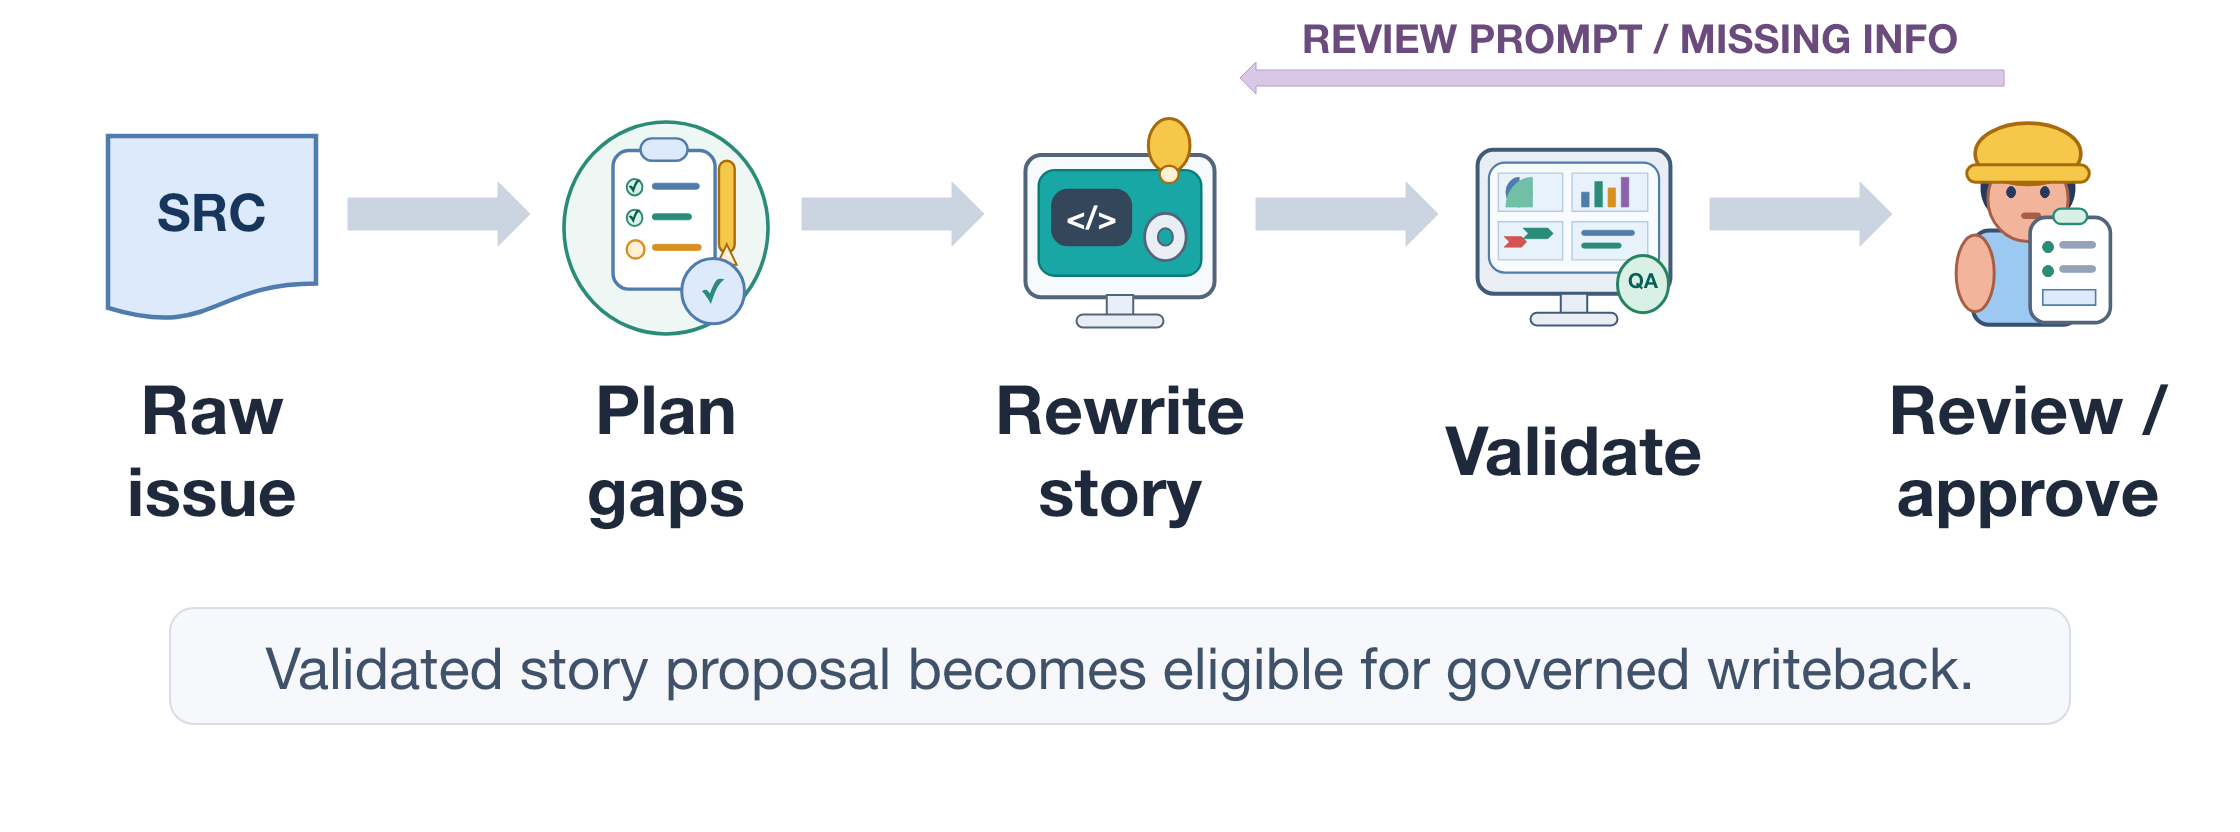
\includegraphics[width=\linewidth]{fig_agentic_module_story_issue_enhancer.png}
\caption{Agentic module 1: story/issue enhancer.}
\label{fig:module-story-issue}
\end{subfigure}
\par\medskip
\begin{subfigure}[t]{0.93\textwidth}
\centering
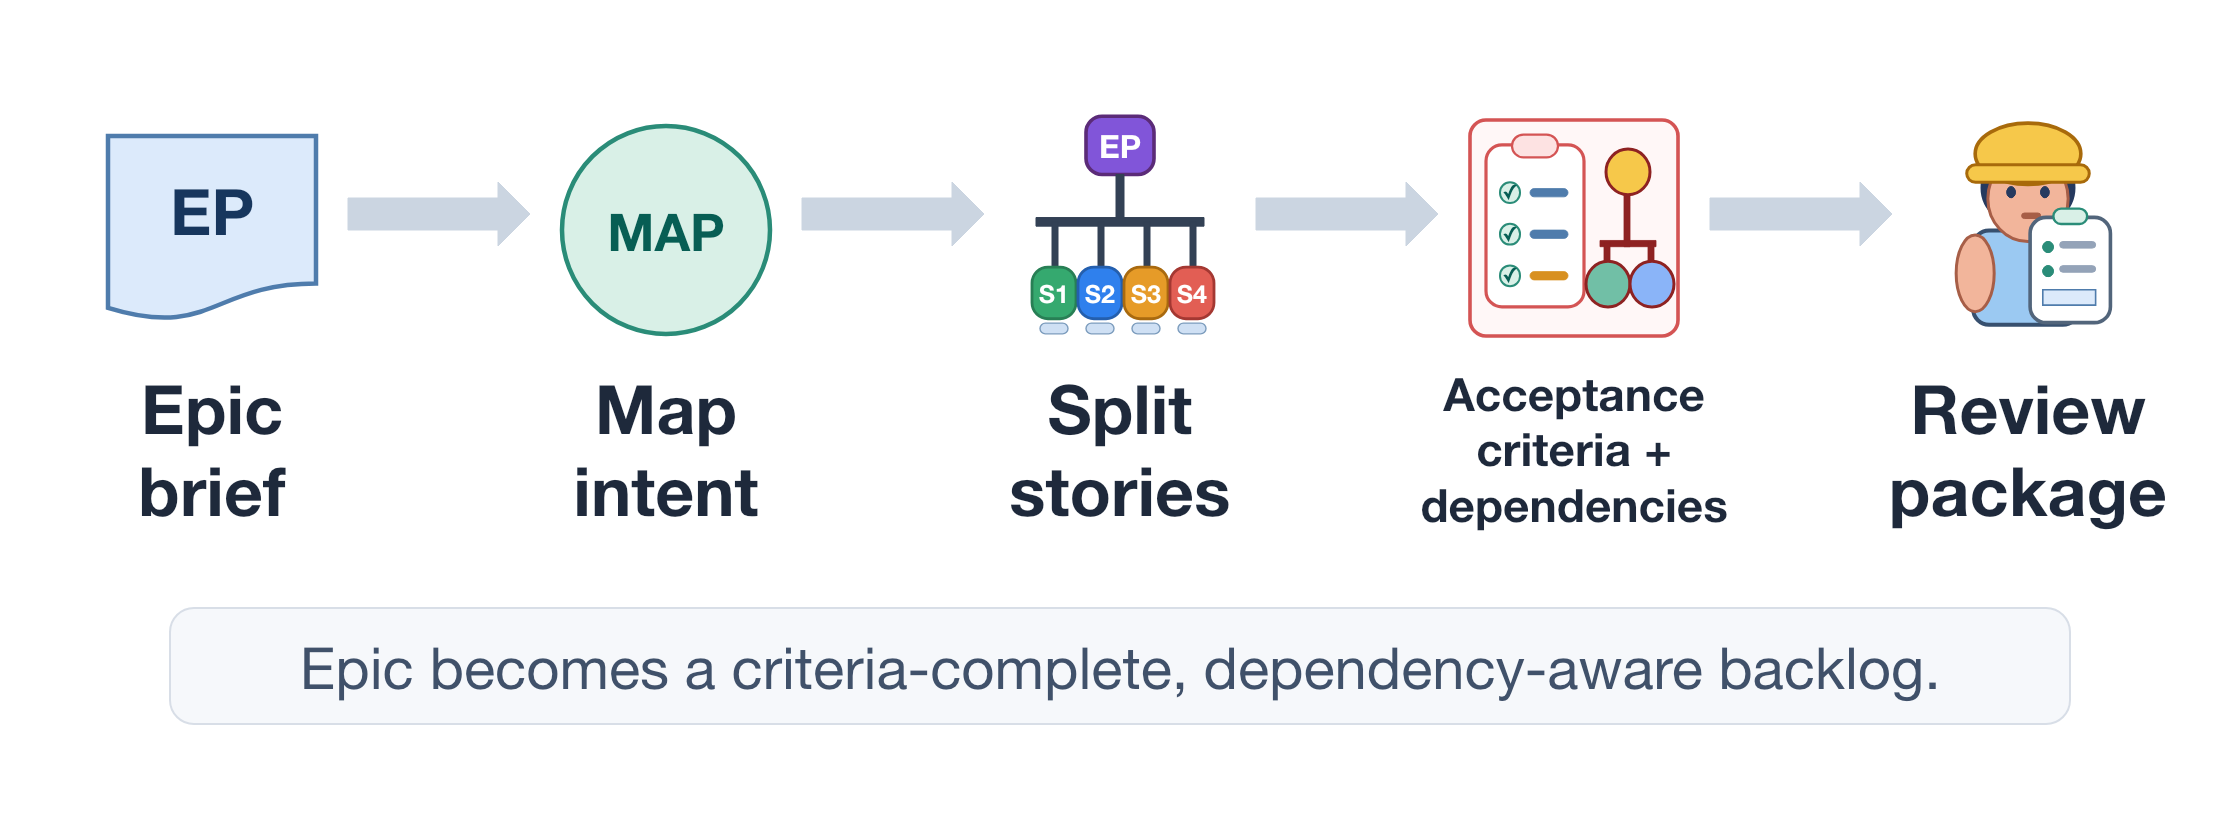
\includegraphics[width=\linewidth]{fig_agentic_module_epic_breaker.png}
\caption{Agentic module 2: epic breaker into stories.}
\label{fig:module-epic-breaker}
\end{subfigure}

\caption{Modular agent architecture: story/issue enhancement, epic-to-story decomposition, prompt-pack creation, and RL-based policy control. The panels expose agent boundaries hidden in the top-level architecture. Panels (c) and (d) continue on the next figure page.}
\label{fig:agentic-module-architecture}
\end{figure*}

\begin{figure*}[p]
\ContinuedFloat
\centering

\begin{subfigure}[t]{0.93\textwidth}
\centering
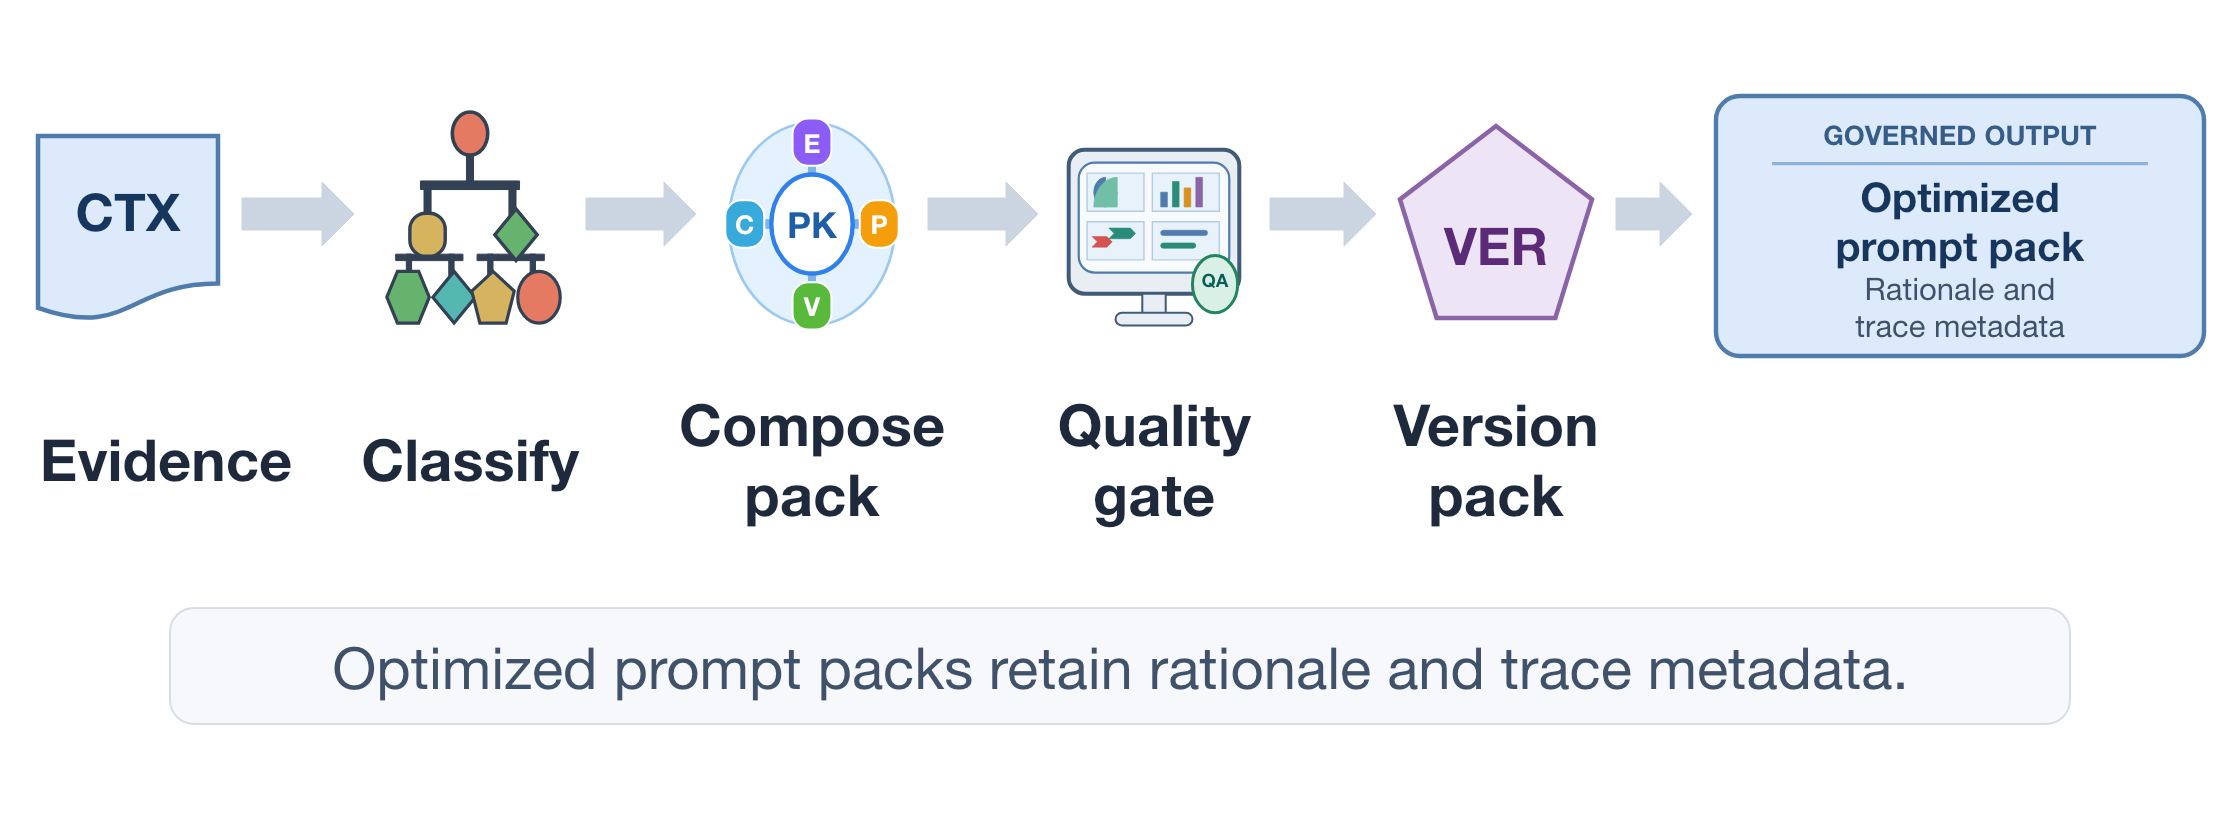
\includegraphics[width=\linewidth]{fig_agentic_module_prompt_generator.png}
\caption{Agentic module 3: prompt generator.}
\label{fig:module-prompt-generator}
\end{subfigure}
\par\medskip
\begin{subfigure}[t]{0.93\textwidth}
\centering
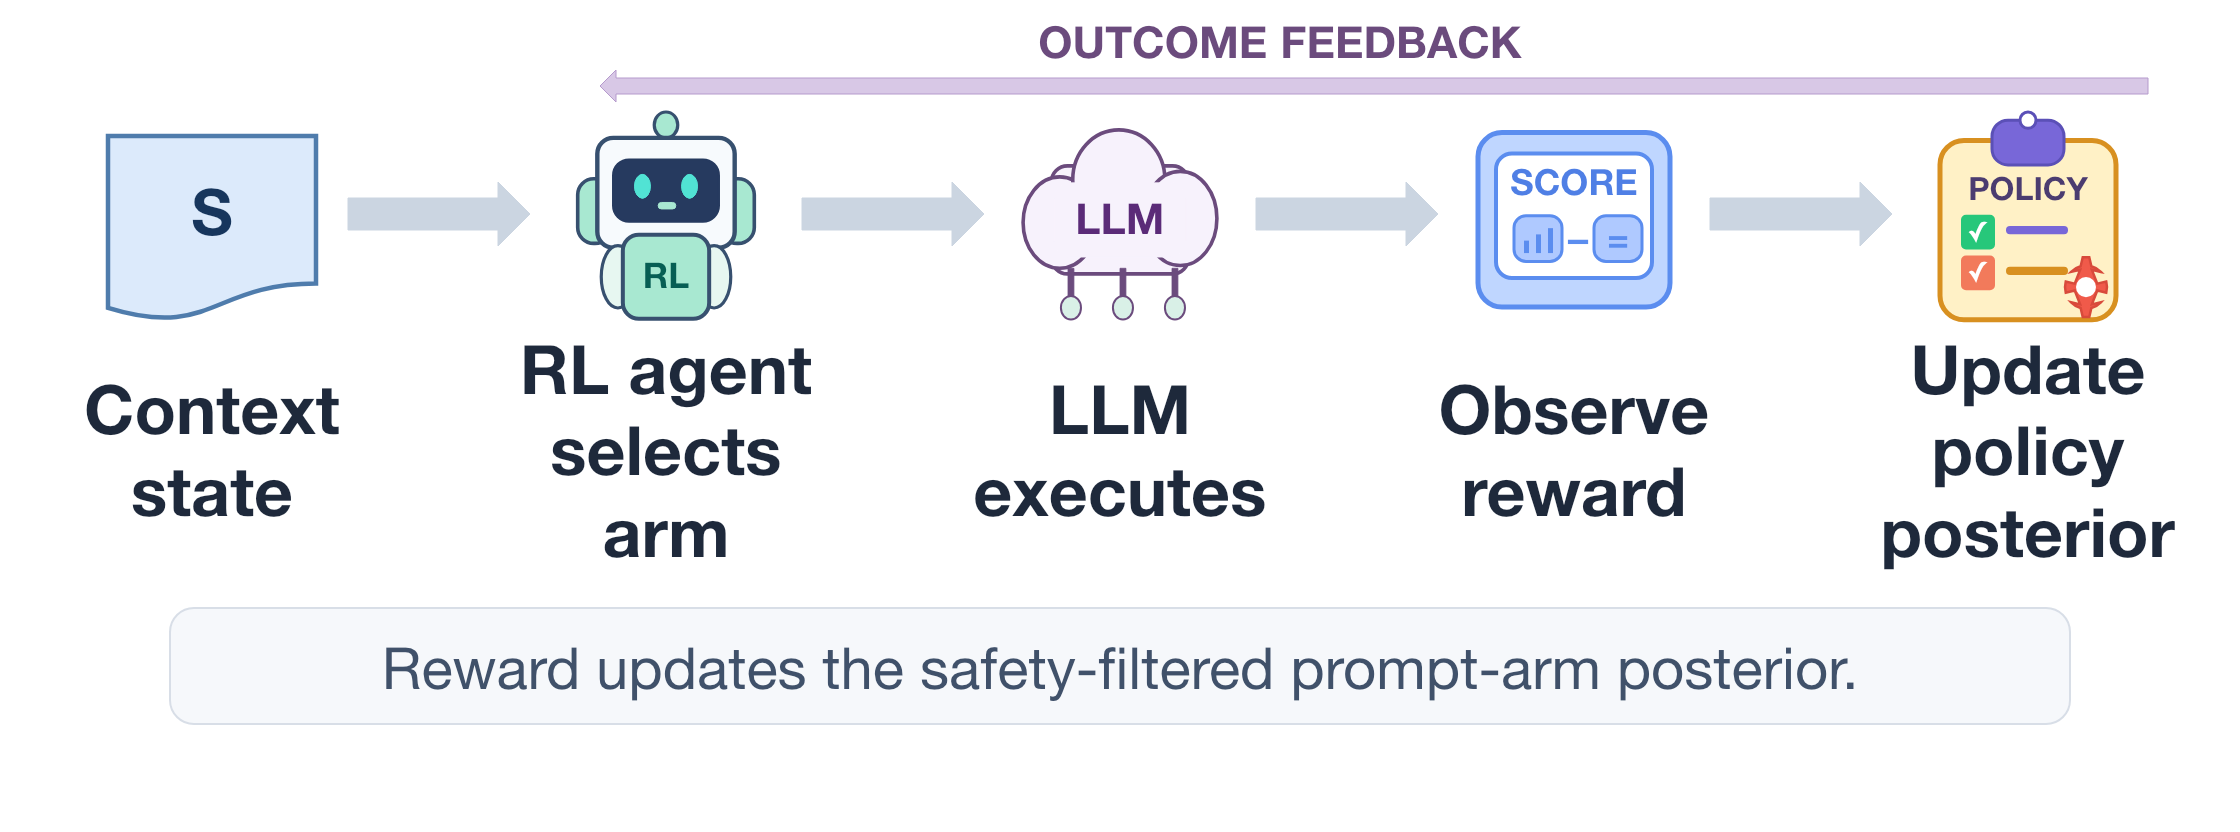
\includegraphics[width=\linewidth]{fig_agentic_module_rl_controller.png}
\caption{Agentic module 4: RL controller.}
\label{fig:module-rl-controller}
\end{subfigure}
\caption{Modular agent architecture (continued): prompt-pack creation and RL-based policy control.}
\Description{Four-panel modular architecture figure showing story issue enhancement, epic-to-story decomposition, prompt generation, and reinforcement-learning controller modules.}

\end{figure*}
\FloatBarrier
\end{document}
